\section*{Exercises}

\begin{ex}
  Consider $\R^3$ with the usual dot product. Let
  \begin{equation*}
    \vect{u}_1 = \begin{mymatrix}{r} -1 \\ 1 \\ 1 \end{mymatrix},
    \quad
    \vect{u}_2 = \begin{mymatrix}{r} -1 \\ -2 \\ 1 \end{mymatrix},
    \quad\mbox{and}\quad
    \vect{v} = \begin{mymatrix}{r} -1 \\ 5 \\ 3 \end{mymatrix}.
  \end{equation*}
  Note that $\vect{u}_1$ and $\vect{u}_2$ are orthogonal.
  Find the best approximation of $\vect{v}$ in $\sspan\set{\vect{u}_1,
    \vect{u}_2}$.
  \begin{sol}
    The best approximation is $\vect{v}' = 3\vect{u}_1 - \vect{u}_2 =
    \begin{mymatrix}{r} -2 \\ 5 \\ 2 \end{mymatrix}$.
  \end{sol}
\end{ex}

\begin{ex}
  Consider $\R^4$ with the usual dot product. Let
  \begin{equation*}
    \vect{u}_1 = \begin{mymatrix}{r} 0 \\ 0 \\ 1 \\ 3 \end{mymatrix},
    \quad
    \vect{u}_2 = \begin{mymatrix}{r} 1 \\ 1 \\ 0 \\ 0 \end{mymatrix},
    \quad
    \vect{u}_3 = \begin{mymatrix}{r} 1 \\ -1 \\ 3 \\ -1 \end{mymatrix},
    \quad\mbox{and}\quad
    \vect{v} = \begin{mymatrix}{r} 6 \\  -2 \\ -5 \\  5 \end{mymatrix}.
  \end{equation*}
  Note that $\vect{u}_1$, $\vect{u}_2$, and $\vect{u}_3$ are
  orthogonal.  Find the best approximation of $\vect{v}$ in
  $\sspan\set{\vect{u}_1,\vect{u}_2, \vect{u}_3}$.
  \begin{sol}
    The best approximation is
    $\vect{v}' = \vect{u}_1 + 2\vect{u}_2 - \vect{u}_3
    = \begin{mymatrix}{r} 1 \\ 3 \\ -2 \\ 4 \end{mymatrix}$.
  \end{sol}
\end{ex}

\begin{ex}
  In the inner product space $V=C[-1,1]$, consider the function
  $f\in V$ given by
  \begin{equation*}
    f(x)
    ~=~ \begin{cases}
      1 & \text{if $x<0$,} \\
      1-x & \text{if $x\geq 0$.}
    \end{cases}
  \end{equation*}
  Find the closest approximation to $f$ by a polynomial of degree at
  most 0, 1, 2, 3, and 4. Graph both $f$ and the approximating
  polynomials.
  \begin{sol}
    Let $p_0,p_1,\ldots$ be the Legendre polynomials from Section~\ref{sec:gram-schmidt}.
    The approximating polynomials are:
    \begin{eqnarray*}
      f_0(x) &=& \frac{3}{4}p_0, \\
      f_1(x) &=& \frac{3}{4}p_0 - \frac{1}{2}p_1, \\
      f_2(x) &=& \frac{3}{4}p_0 - \frac{1}{2}p_1 - \frac{15}{32}p_2, \\
      f_3(x) &=& \frac{3}{4}p_0 - \frac{1}{2}p_1 - \frac{15}{32}p_2 + 0p_3, \\
      f_4(x) &=& \frac{3}{4}p_0 - \frac{1}{2}p_1 - \frac{15}{32}p_2 + 0p_3 + \frac{105}{256}p_4.
    \end{eqnarray*}
    \begin{center}
      \definecolor{my-yellow}{rgb}{1.00,0.87,0.00}
      \definecolor{my-green}{rgb}{0,1,0}
      \definecolor{my-lightblue}{rgb}{0,0.7,0.9}
      \definecolor{my-blue}{rgb}{0,0,0.9}
      \definecolor{my-red}{rgb}{1,0.3,0}
      \definecolor{my-gray}{rgb}{0.4,0.4,0.4}
      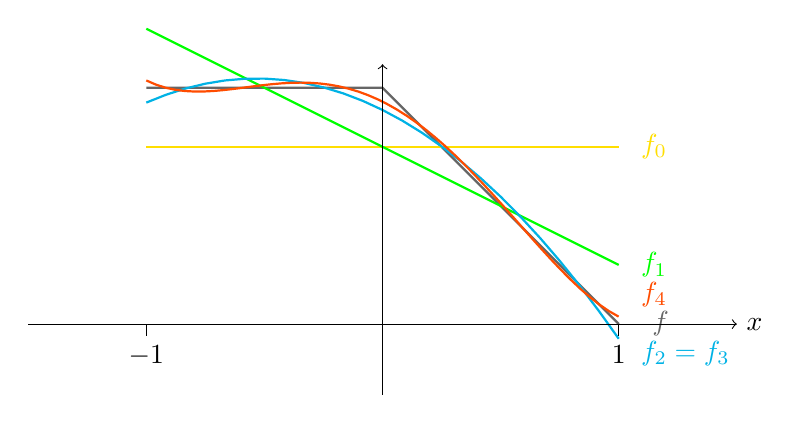
\begin{tikzpicture}[domain=-1:1, scale=3, samples=25]
        \def\fA#1{1}
        \def\fB#1{(#1)}
        \def\fC#1{(abs((#1)^2)-1/3)}
        \def\fD#1{((#1)^3-3/5*(#1))}
        \def\fE#1{(abs((#1)^4)-6/7*abs((#1)^2)+3/35)}
        \def\fF#1{((#1)^5 - 10/9*(#1)^3+5/21*(#1))}
        \def\fG#1{(abs((#1)^6)-15/11*abs((#1)^4)+5/11*abs((#1)^2)-5/231)}
        \def\fH#1{((429*(#1)^7 - 693*(#1)^5 + 315*(#1)^3 - 35*(#1))/429)}
        \def\fI#1{((6435*abs((#1)^8)-12012*abs((#1)^6)+6930*abs((#1)^4)-1260*abs((#1)^2)+35)/6435)}
        \draw[thick,color=my-gray] (-1,1) -- (0,1) -- (1,0);
        \path[color=my-gray] (1,0) node[right=2ex] {$f$};
        \draw[thick,color=my-yellow]         plot (\x,{0.75*\fA{\x}}) (1,0.75) node[right=1ex] {$f_0$};
        \draw[thick,color=my-green]          plot (\x,{0.75*\fA{\x} - 0.5*\fB{\x}}) (1,0.25) node[right=1ex] {$f_1$};
        \draw[thick,color=my-lightblue]      plot (\x,{0.75*\fA{\x} - 0.5*\fB{\x} - 15/32*\fC{\x}}) (1,-0.125) node[right=1ex] {$f_2=f_3$};
        \draw[thick,color=my-red,samples=50] plot (\x,{0.75*\fA{\x} - 0.5*\fB{\x} - 15/32*\fC{\x} + 105/256*\fE{\x}}) (1,0.125) node[right=1ex] {$f_4$};
        \draw[->] (-1.5,0) -- (1.5,0) node[right] {$x$};
        \draw[->] (0,-0.3) -- (0,1.1);
        \draw (1,0) -- (1,-0.05) node[below] {$1$};
        \draw (-1,0) -- (-1,-0.05) node[below] {$-1$};
      \end{tikzpicture}
    \end{center}
  \end{sol}
\end{ex}

\begin{ex}
  In the inner product space $C[-\pi,\pi]$, consider the orthogonal
  set of functions from Example~\ref{exa:orthogonal-set-sin-cos}:
  $\set{1, \sin x, \cos x, \sin 2x, \cos 2x, \sin 3x, \cos 3x, \ldots}$.  Let
  $f(x) = x^2$, where $x\in[-\pi,\pi]$. Find the Fourier series of
  $f$.
  \begin{sol}
    $\frac{\pi^2}{3} - \frac{4}{1}\cos x + \frac{4}{4}\cos 2x - \frac{4}{9} \cos 3x + \frac{4}{16} \cos 4x - \frac{4}{25} \cos 5x \pm \ldots$.
  \end{sol}
\end{ex}
